\documentclass[10pt, aspectratio=169, handout]{beamer}
\usefonttheme{professionalfonts}

\mode<presentation>
{
  \usetheme{Berkeley}
  \usecolortheme{beaver}
  \usefonttheme{default}
  \setbeamertemplate{navigation symbols}{}
  \setbeamertemplate{caption}[numbered]
} 

\setbeamertemplate{footline}{%
  \leavevmode%
  \hbox{%
    \begin{beamercolorbox}[wd=.85\paperwidth,ht=2.5ex,dp=1ex,left]{author in head/foot}%
      \usebeamerfont{author in head/foot}Maxx Seminario, Electronic Circuits, Spring 2026%
    \end{beamercolorbox}%
    \begin{beamercolorbox}[wd=.15\paperwidth,ht=2.5ex,dp=1ex,right]{date in head/foot}%
      \hspace*{0.5em}\insertframenumber{} / \inserttotalframenumber\hspace*{0.5em}%
    \end{beamercolorbox}%
  }%
  \vskip0pt%
}


\usepackage[english]{babel}
\usepackage[utf8]{inputenc}
\usepackage{tikz}
\usepackage{pgfplots}
\usepackage{array}
\usepackage{makecell}
\usepackage{verbatim}
\usepackage{graphicx}
\usepackage{subcaption}
\usepackage{amsfonts}
\usepackage{amsmath}
\usepackage{bm}
\usepackage{epstopdf}
\usepackage[american]{circuitikz}
\usepackage{caption}
\captionsetup{compatibility=false}
\usepackage[absolute,overlay]{textpos}
\usetikzlibrary{calc}
\usetikzlibrary{pgfplots.fillbetween, backgrounds}
\usetikzlibrary{positioning}
\usetikzlibrary{pgfplots.groupplots}
\usetikzlibrary{plotmarks}
\usetikzlibrary{calc}
\usetikzlibrary{decorations.markings}
\usetikzlibrary{arrows.meta}

\usepgfplotslibrary{groupplots}
\pgfplotsset{compat=newest} 

% \usepackage{ifthen}
% \newboolean{showresults}
% \setboolean{showresults}{false}

\usepackage{hyperref}
\hypersetup{
    colorlinks=true,
    linkcolor=blue,
    filecolor=magenta,      
    urlcolor=cyan,
}

% Added by Maxx Seminario 01/06/2026 - for colored icons in itemize labels
\usepackage{wasysym} % for smiles and frowns
\newcommand{\neutralface}{%
  \tikz[baseline=-0.6ex]{
    \draw (0,0) circle (0.9ex);
    \fill (-0.35ex,0.25ex) circle (0.12ex);
    \fill ( 0.35ex,0.25ex) circle (0.12ex);
    \draw (-0.35ex,-0.25ex) -- (0.35ex,-0.25ex);
  }%
}
\newcommand{\baditem}{\textcolor{red!70!black}{\frownie}}
\newcommand{\gooditem}{\textcolor{green!60!black}{\smiley}}
\newcommand{\mehitem}{\textcolor{orange!80!black}{\neutralface}}

\title[ECEN 222]{Frequency Domain Analysis of Circuits}
\author{Maxx Seminario}
\institute{University of Nebraska-Lincoln}
\date{Spring 2026}

\begin{document}
\begin{frame}
  \titlepage
\end{frame}

\section{Introduction to Frequency Domain}

\begin{frame}{Why Frequency Domain Analysis?}
    
    \begin{columns}[t]
    \column{0.48\textwidth}
        \textbf{Limitations of Time Domain}:
        \begin{itemize}
            \item Differential equations for AC circuits
            \item Complex trig math
            \item Difficult for sinusoidal steady-state
        \end{itemize}
        
        \textbf{Frequency Domain Advantages}:
        \begin{itemize}
            \item Converts differential equations to algebra
            \item Easy handling of sinusoidal signals
            \item Simplifies AC circuit analysis
        \end{itemize}
        
    \column{0.48\textwidth}
        \textbf{Applications}:
        \begin{itemize}
            \item AC power systems (60 Hz)
            \item Audio systems (20 Hz - 20 kHz)
            \item Radio frequency circuits (MHz - GHz)
            \item Signal processing and filtering
        \end{itemize}
        
        \begin{block}{Domain Transformation Tool}
            \textbf{Phasor transform} converts time-domain sinusoids to frequency-domain complex numbers
        \end{block}
        
    \end{columns}
    
    \begin{alertblock}{Goal for this lecture}
        Review frequency domain (phasor) analysis for AC circuits
    \end{alertblock}
    
\end{frame}

\begin{frame}{Sinusoidal Signals:  The Foundation}
    
    \begin{columns}[t]
    \column{0.48\textwidth}
        \textbf{General Sinusoidal Signal}: 
        \[
        v(t) = V_m \cos(\omega t + \phi)
        \]
        
        where: 
        \begin{itemize}
            \item $V_m$ = amplitude (peak value)
            \item $\omega$ = angular frequency (rad/s)
            \item $\phi$ = phase angle (radians or degrees)
        \end{itemize}
        
        \vspace{0.5cm}
        
        \textbf{Related Parameters}:
        \begin{itemize}
            \item Frequency: $f = \omega/(2\pi)$ (Hz)
            \item Period: $T = 1/f = 2\pi/\omega$ (s)
            \item RMS value: $V_{rms} = V_m/\sqrt{2}$
        \end{itemize}
        
    \column{0.48\textwidth}
        \textbf{Sinusoidal Waveform}:
        
        \begin{figure}[htb]
        \centering
        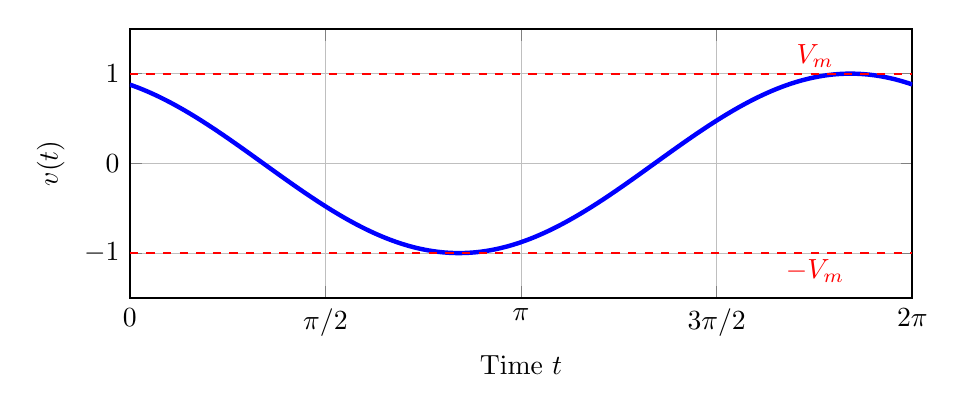
\begin{tikzpicture}
            \begin{axis}[
                width=0.95\textwidth,
                height=5cm,
                xlabel={Time $t$},
                ylabel={$v(t)$},
                xmin=0, xmax=6.28,
                ymin=-1.5, ymax=1.5,
                grid=major,
                xtick={0, 1.57, 3.14, 4.71, 6.28},
                xticklabels={0, $\pi/2$, $\pi$, $3\pi/2$, $2\pi$},
                thick
            ]
            \addplot[blue, ultra thick, domain=0:6.28, samples=200] 
                {cos(deg(x + 0.5))};
            
            % Amplitude markers
            \draw[dashed, red] (axis cs:0,1) -- (axis cs:6.28,1);
            \draw[dashed, red] (axis cs:0,-1) -- (axis cs:6.28,-1);
            \node[red] at (axis cs: 5.5,1.2) {$V_m$};
            \node[red] at (axis cs:5.5,-1.2) {$-V_m$};
            \end{axis}
        \end{tikzpicture}
        \end{figure}
        
    \end{columns}
    
\end{frame}

\section{Phasor Representation}

\begin{frame}{Phasor Concept:  From Time to Frequency Domain}
    
    \begin{columns}[t]
    \column{0.48\textwidth}
        \textbf{Euler's Identity}:
        \[
        e^{j\theta} = \cos\theta + j\sin\theta
        \]
        
        \textbf{Sinusoid as Complex Exponential}:
        \[
        v(t) = V_m \cos(\omega t + \phi)
        \]
        \[
        v(t) = \text{Re}\{V_m e^{j(\omega t + \phi)}\}
        \]
        \[
        v(t) = \text{Re}\{V_m e^{j\phi} e^{j\omega t}\}
        \]
        
        \begin{block}{Phasor Definition}
            \[
            \mathbf{V} = V_m e^{j\phi} = V_m \angle \phi
            \]
        \end{block}
        
    \column{0.48\textwidth}
        \textbf{Phasor Diagram}:
        
        \begin{figure}[htb]
        \centering
        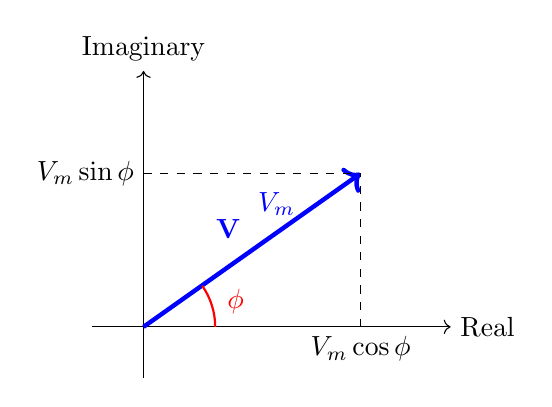
\begin{tikzpicture}[scale=1.3]
            % Axes
            \draw[->] (-0.5,0) -- (3,0) node[right] {Real};
            \draw[->] (0,-0.5) -- (0,2.5) node[above] {Imaginary};
            
            % Phasor
            \draw[->, ultra thick, blue] (0,0) -- (2.121,1.5) node[midway, above left] {$\mathbf{V}$};
            
            % Angle
            \draw[red, thick] (0.7,0) arc (0:35: 0.7);
            \node[red] at (0.9,0.25) {$\phi$};
            
            % Components
            \draw[dashed] (2.121,0) -- (2.121,1.5);
            \draw[dashed] (0,1.5) -- (2.121,1.5);
            \node[below] at (2.121,0) {$V_m\cos\phi$};
            \node[left] at (0,1.5) {$V_m\sin\phi$};
            
            % Magnitude label
            \node[blue] at (1.3,1.2) {$V_m$};
        \end{tikzpicture}
        \end{figure}
        
        \vspace{-0.1cm}
        
        \textbf{Rectangular Form}:
        \[
        \mathbf{V} = V_m\cos\phi + jV_m\sin\phi
        \]
        
    \end{columns}
    
\end{frame}

\begin{frame}{Phasor Transform:  Summary}
    
    \begin{table}
    \centering
    \renewcommand{\arraystretch}{2.0}
    \begin{tabular}{|c|c|c|}
    \hline
    \textbf{Time Domain} & \textbf{Phasor Domain} & \textbf{Operation} \\
    \hline
    \hline
    $V_m \cos(\omega t + \phi)$ & $\mathbf{V} = V_m \angle \phi$ & Domain transformation \\
    \hline
    $\dfrac{d}{dt}$ & $j\omega$ & Differentiation $\rightarrow$ multiplication \\
    \hline
    $\displaystyle\int dt$ & $\dfrac{1}{j\omega}$ & Integration $\rightarrow$ division \\
    \hline
    Addition & Addition & Same (LTI Systems) \\
    \hline
    \end{tabular}
    \end{table}
    
    % \vspace{0.5cm}
    
    \begin{block}{Key Advantage}
        \begin{itemize}
            \item[\gooditem] \textbf{Differentiation} in time domain $\rightarrow$ \textbf{Multiplication} by $j\omega$ in phasor domain.
            \item[\mehitem] Phasor analysis only works for \textbf{linear circuits} with \textbf{sinusoidal sources} at the \textbf{same frequency} in \textbf{steady-state}
        \end{itemize}


        
    \end{block}
    
\end{frame}

\section{Impedance}

\begin{frame}{Electrical Impedance}
    
    \begin{columns}[t]
    \column{0.48\textwidth}
        \textbf{Definition}:
        
        Impedance is the ratio of phasor voltage to phasor current:
        \[
        \mathbf{Z} = \frac{\mathbf{V}}{\mathbf{I}}
        \]
        
        \vspace{-0.3cm}
        
        \textbf{Polar Form}:
        \[
        \mathbf{Z} = |\mathbf{Z}| \angle \theta
        \]
        
        \textbf{Rectangular Form}: 
        \[
        \mathbf{Z} = R + jX
        \]
        where: 
        \begin{itemize}
            \item $R$ = resistance (real part)
            \item $X$ = reactance (imaginary part)
        \end{itemize}
        
    \column{0.48\textwidth}
        \textbf{Impedance in Complex Plane}:
        
        \begin{figure}[htb]
        \centering
        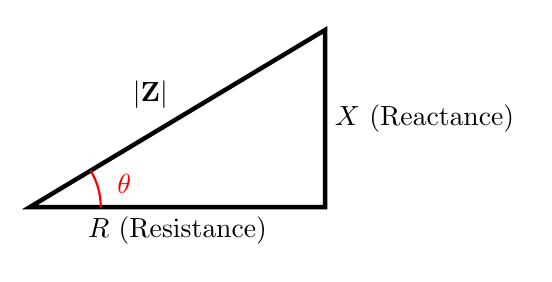
\begin{tikzpicture}[scale=1.5]
            % Triangle
            \draw[ultra thick] (0,0) -- (2.5,0) -- (2.5,1.5) -- cycle;
            
            % Labels
            \node[below] at (1.25,0) {$R$ (Resistance)};
            \node[right] at (2.5,0.75) {$X$ (Reactance)};
            \node[above left] at (1.25,0.75) {$|\mathbf{Z}|$};
            
            % Angle
            \draw[red, thick] (0.6,0) arc (0:31: 0.6);
            \node[red] at (0.8,0.2) {$\theta$};
        \end{tikzpicture}
        \end{figure}
        
        \textbf{Relationships}:
        \[
        |\mathbf{Z}| = \sqrt{R^2 + X^2}
        \]
        \[
        \theta = \tan^{-1}\left(\frac{X}{R}\right)
        \]
        
    \end{columns}
    
\end{frame}

\begin{frame}{Impedance of R, L, and C}
    
    \begin{table}
    \centering
    \renewcommand{\arraystretch}{2.2}
    \begin{tabular}{|c|c|c|c|}
    \hline
    \textbf{Element} & \textbf{Time Domain} & \textbf{Impedance} & \textbf{Phase} \\
    \hline
    \hline
    Resistor & $v = iR$ & $\mathbf{Z}_R = R$ & $0°$ \\
    \hline
    Inductor & $v = L\dfrac{di}{dt}$ & $\mathbf{Z}_L = j\omega L$ & $+90°$ \\
    \hline
    Capacitor & $i = C\dfrac{dv}{dt}$ & $\mathbf{Z}_C = \dfrac{1}{j\omega C} = \dfrac{-j}{\omega C}$ & $-90°$ \\
    \hline
    \end{tabular}
    \end{table}
    
    \vspace{0.5cm}
    
    \begin{columns}[t]
    \column{0.32\textwidth}
        \textbf{Resistor}:
        \begin{itemize}
            \item Real impedance
            \item V and I in phase
            \item Frequency independent
        \end{itemize}
        
    \column{0.32\textwidth}
        \textbf{Inductor}:
        \begin{itemize}
            \item Imaginary impedance
            \item V leads I by 90°
            \item $|\mathbf{Z}_L| = \omega L$ increases with $\omega$
        \end{itemize}
        
    \column{0.32\textwidth}
        \textbf{Capacitor}: 
        \begin{itemize}
            \item Imaginary impedance
            \item I leads V by 90°
            \item $|\mathbf{Z}_C| = 1/(\omega C)$ decreases with $\omega$
        \end{itemize}
        
    \end{columns}
    
\end{frame}

\begin{frame}{Frequency Behavior of Impedance}
    
    \begin{figure}[htb]
    \centering
    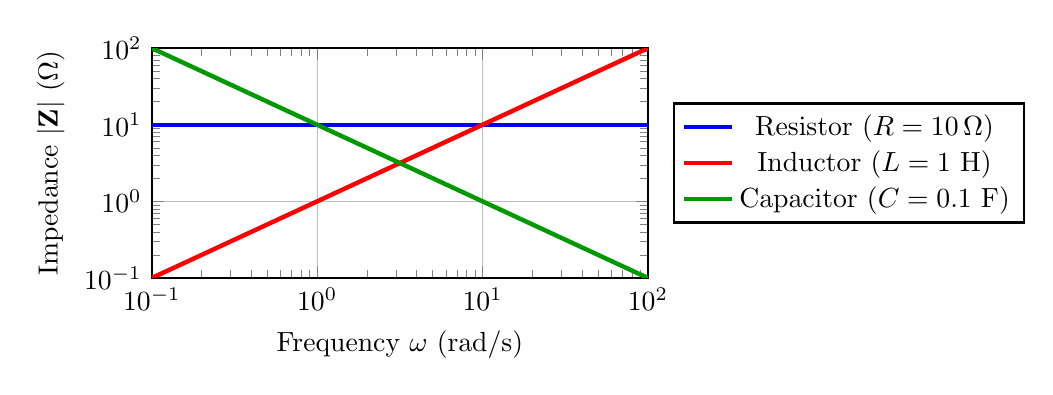
\begin{tikzpicture}
        \begin{axis}[
            width=0.65\textwidth,
            height=4.5cm,
            xlabel={Frequency $\omega$ (rad/s)},
            ylabel={Impedance $|\mathbf{Z}|$ ($\Omega$)},
            xmin=0.1, xmax=100,
            ymin=0.1, ymax=100,
            xmode=log,
            ymode=log,
            grid=major,
            legend style={at={(1.05,0.5)}, anchor=west},
            thick
        ]
        % Resistor (constant)
        \addplot[blue, ultra thick, domain=0.1:100] {10};
        \addlegendentry{Resistor ($R = 10\,\Omega$)}
        
        % Inductor (increasing)
        \addplot[red, ultra thick, domain=0.1:100] {x};
        \addlegendentry{Inductor ($L = 1$ H)}
        
        % Capacitor (decreasing)
        \addplot[green! 60! black, ultra thick, domain=0.1:100] {10/x};
        \addlegendentry{Capacitor ($C = 0.1$ F)}
        \end{axis}
    \end{tikzpicture}
    \end{figure}

    \vspace{-0.6cm}
    
    \begin{block}{Frequency Behavior}
        \begin{itemize}
            \item \textbf{Resistor}: Constant impedance (frequency independent)
            \item \textbf{Inductor}: High impedance at high frequencies (blocks AC, passes DC)
            \item \textbf{Capacitor}: Low impedance at high frequencies (blocks DC, passes AC)
        \end{itemize}
    \end{block}
    
\end{frame}

\section{Phasor Circuit Analysis}

\begin{frame}{Phasor Analysis:  Circuit Laws}
    
    \textbf{All DC circuit analysis techniques apply to phasors }
    
    \vspace{0.5cm}
    
    \begin{columns}[t]
    \column{0.48\textwidth}
        \textbf{Kirchhoff's Voltage Law (KVL)}:
        \[
        \sum \mathbf{V}_k = 0
        \]
        
        \textbf{Kirchhoff's Current Law (KCL)}:
        \[
        \sum \mathbf{I}_k = 0
        \]
        
        \textbf{Ohm's Law}:
        \[
        \mathbf{V} = \mathbf{I} \mathbf{Z}
        \]
        
    \column{0.48\textwidth}
        \textbf{Series Impedances}:
        \[
        \mathbf{Z}_{eq} = \mathbf{Z}_1 + \mathbf{Z}_2 + \cdots + \mathbf{Z}_n
        \]
        
        \textbf{Parallel Impedances}:
        \[
        \mathbf{Z}_{eq}^{-1} = \mathbf{Z}_{1}^{-1} + \mathbf{Z}_{2}^{-1} + \cdots + \mathbf{Z}_{n}^{-1}
        \]
        
        \textbf{Voltage Divider}:
        \[
        \mathbf{V}_k = \mathbf{V}_s \mathbf{Z}_k(\mathbf{Z}_1 + \mathbf{Z}_2)^{-1}
        \]
        
    \end{columns}
    
    \begin{alertblock}{Key Point}
        Replace resistances with impedances, and voltages/currents with phasors.  Then use the standard DC techniques
    \end{alertblock}
    
\end{frame}

\begin{frame}{Example: Series RC Circuit}
    
    \begin{columns}[t]
    \column{0.48\textwidth}
        \textbf{Circuit}:
        
        \begin{figure}[htb]
        \centering
        \begin{circuitikz}[scale=0.8]
            \draw (0,0) to[sinusoidal voltage source, l=$v_s(t)$] (0,3);
            \draw (0,3) to[R, l=$R$, i^=$i(t)$] (3,3);
            \draw (3,3) to[C, l_=$C$, v^=$v_C(t)$] (3,0);
            \draw (3,0) to[short] (0,0);
        \end{circuitikz}
        \end{figure}
        
        \textbf{Given}:
        \begin{itemize}
            \item $v_s(t) = V_m \cos(\omega t)$
            \item $R = 100\,\Omega$
            \item $C = 10\,\mu$F
            \item $\omega = 1000$ rad/s
        \end{itemize}
        
    \column{0.48\textwidth}
        \textbf{Phasor Analysis}:
        
        Source phasor: $\mathbf{V}_s = V_m \angle 0°$
        
        Impedances:
        \[
        \mathbf{Z}_R = 100\,\Omega
        \]
        \[
        \mathbf{Z}_C = \frac{-j}{\omega C} = \frac{-j}{0.01} = -j100\,\Omega
        \]
        
        Total impedance:
        \[
        \mathbf{Z}_{eq} = R - jX_C = 100 - j100
        \]
        \[
        = 141.4 \angle -45° \,\Omega
        \]
        
        \vspace{-0.2cm}
        
        Current: 
        \[
        \mathbf{I} = \frac{\mathbf{V}_s}{\mathbf{Z}_{eq}} = \frac{V_m \angle 0°}{141.4 \angle -45°} = \frac{V_m}{141.4} \angle 45°
        \]
        
    \end{columns}
    
\end{frame}

\begin{frame}{Example: Phasor Diagram}
    
    \begin{columns}[t]
    \column{0.48\textwidth}
        \textbf{Voltage Divider}:
        
        Capacitor voltage: 
        \[
        \mathbf{V}_C = \mathbf{V}_s \frac{\mathbf{Z}_C}{\mathbf{Z}_R + \mathbf{Z}_C}
        \]
        \[
        = \mathbf{V}_s \frac{-j100}{100 - j100}
        \]
        \[
        = \mathbf{V}_s \frac{100 \angle -90°}{141.4 \angle -45°}
        \]
        \[
        = 0.707 V_m \angle -45°
        \]
        
        \vspace{0.3cm}
        
        Resistor voltage:
        \[
        \mathbf{V}_R = \mathbf{I} R = 0.707 V_m \angle 45°
        \]
        
    \column{0.48\textwidth}
        \textbf{Phasor Diagram}: 
        
        \begin{figure}[htb]
        \centering
        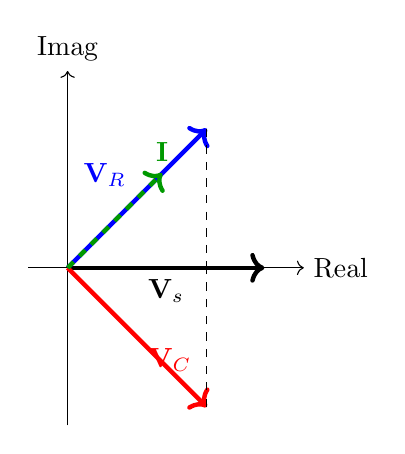
\begin{tikzpicture}[scale=1.0]
            % Axes
            \draw[->] (-0.5,0) -- (3,0) node[right] {Real};
            \draw[->] (0,-2) -- (0,2.5) node[above] {Imag};
            
            % Vs
            \draw[->, ultra thick, black] (0,0) -- (2.5,0) node[midway, below] {$\mathbf{V}_s$};
            
            % VR
            \draw[->, ultra thick, blue] (0,0) -- (1.768,1.768) node[midway, above left] {$\mathbf{V}_R$};
            
            % VC
            \draw[->, ultra thick, red] (0,0) -- (1.768,-1.768) node[midway, below right] {$\mathbf{V}_C$};
            
            % I (parallel to VR)
            \draw[->, ultra thick, green! 60! black, dashed] (0,0) -- (1.2,1.2) node[above] {$\mathbf{I}$};
            
            % Annotations
            \draw[dashed] (1.768,1.768) -- (1.768,0);
            \draw[dashed] (1.768,-1.768) -- (1.768,0);
        \end{tikzpicture}
        \caption{$\mathbf{V}_R + \mathbf{V}_C = \mathbf{V}_s$ (KVL)}
        \end{figure}
        
    \end{columns}
    
\end{frame}

\begin{frame}{Example: Series RLC Circuit}
    
    \begin{columns}[t]
    \column{0.48\textwidth}
        \textbf{Circuit}:
        
        \begin{figure}[htb]
        \centering
        \begin{circuitikz}[scale=0.85]
            \draw (0,0) to[sinusoidal voltage source, l=$v_s(t)$] (0,3);
            \draw (0,3) to[R, l=$R$] (1.5,3);
            \draw (1.5,3) to[L, l=$L$] (3,3);
            \draw (3,3) to[C, l=$C$] (3,0);
            \draw (3,0) to[short] (0,0);
        \end{circuitikz}
        \end{figure}
        
        \vspace{-0.3cm}
        
        \textbf{Total Impedance}:
        \[
        \mathbf{Z} = R + j\omega L + \frac{1}{j\omega C} = R + j\left(\omega L - \frac{1}{\omega C}\right)
        \]
        \[
        = R + j(X_L - X_C)
        \]
        
    \column{0.48\textwidth}
        \textbf{Three Cases}:
        
        \textbf{1.  Inductive} ($X_L > X_C$):
        \begin{itemize}
            \item Net reactance is positive
            \item Voltage leads current
            \item Behaves like RL circuit
        \end{itemize}
        
        \textbf{2. Capacitive} ($X_L < X_C$):
        \begin{itemize}
            \item Net reactance is negative
            \item Current leads voltage
            \item Behaves like RC circuit
        \end{itemize}
        
        \textbf{3. Resonant} ($X_L = X_C$):
        \begin{itemize}
            \item Net reactance is zero
            \item $\mathbf{Z} = R$ (purely resistive)
            \item V and I in phase
        \end{itemize}
        
    \end{columns}
    
\end{frame}

\begin{frame}{Resonance in RLC Circuits}
    
    \begin{columns}[t]
    \column{0.48\textwidth}
        \textbf{Resonance Condition}:
        
        At resonance:  $X_L = X_C$
        \[
        \omega_0 L = \frac{1}{\omega_0 C}
        \]
        
        \begin{block}{Resonant Frequency}
            \[
            \omega_0 = \frac{1}{\sqrt{LC}}
            \]
        \end{block}
        
        \textbf{At Resonance}:
        \begin{itemize}
            \item $\mathbf{Z} = R$ (minimum impedance)
            \item Maximum current
            \item Zero phase angle
            \item Energy oscillates between L and C
        \end{itemize}
        
    \column{0.48\textwidth}
        \textbf{Impedance vs.  Frequency}:
        
        \begin{figure}[htb]
        \centering
        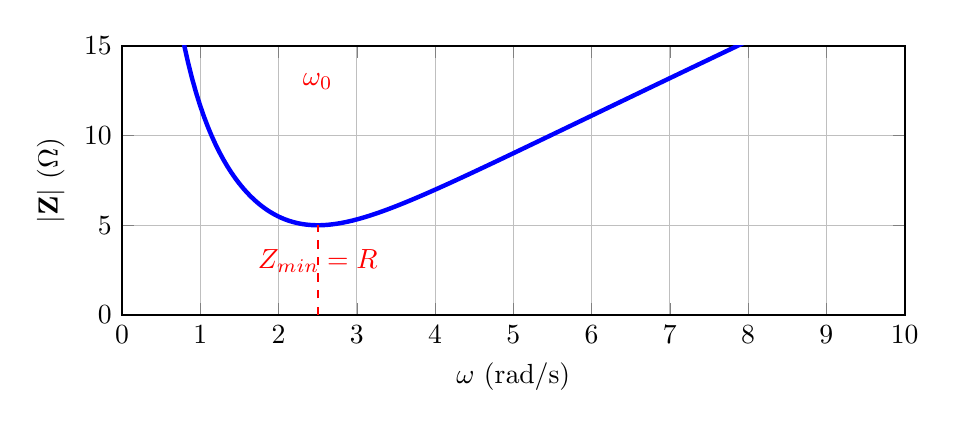
\begin{tikzpicture}
            \begin{axis}[
                width=0.95\textwidth,
                height=5cm,
                xlabel={$\omega$ (rad/s)},
                ylabel={$|\mathbf{Z}|$ ($\Omega$)},
                xmin=0, xmax=10,
                ymin=0, ymax=15,
                grid=major,
                thick
            ]
            % Impedance magnitude
            \addplot[blue, ultra thick, domain=0.1:10, samples=200] 
                {sqrt(25 + (2*x - 12.5/x)^2)};
            
            % Mark resonance
            \draw[dashed, red] (axis cs: 2.5,0) -- (axis cs:2.5,5);
            \node[red] at (axis cs:2.5,13) {$\omega_0$};
            \node[red] at (axis cs:2.5,3) {$Z_{min} = R$};
            \end{axis}
        \end{tikzpicture}
        \end{figure}
        
    \end{columns}
    
\end{frame}

\section{AC Power Analysis}

\begin{frame}{AC Power:  Instantaneous and Average}
    
    \begin{columns}[t]
    \column{0.48\textwidth}
        \textbf{Instantaneous Power}:
        
        For $v(t) = V_m \cos(\omega t)$ and $i(t) = I_m \cos(\omega t - \theta)$:
        \[
        p(t) = v(t) \cdot i(t)
        \]
        \[
        = V_m I_m \cos(\omega t) \cos(\omega t - \theta)
        \]
        
        Using trig identity: 
        \[
        p(t) = \frac{V_m I_m}{2}\cos\theta + \frac{V_m I_m}{2}\cos(2\omega t - \theta)
        \]
        
        \vspace{0.3cm}
        
        \textbf{Average Power}:
        \[
        P = \frac{1}{T}\int_0^T p(t)\,dt = \frac{V_m I_m}{2}\cos\theta
        \]
        
    \column{0.48\textwidth}
        \textbf{Using RMS Values}:
        
        \[
        V_{rms} = \frac{V_m}{\sqrt{2}}, \quad I_{rms} = \frac{I_m}{\sqrt{2}}
        \]
        
        \begin{block}{Average (Real) Power}
            \[
            P = V_{rms} I_{rms} \cos\theta
            \]
        \end{block}
        
        \vspace{-0.2cm}
    
        \begin{figure}[htb]
        \centering
        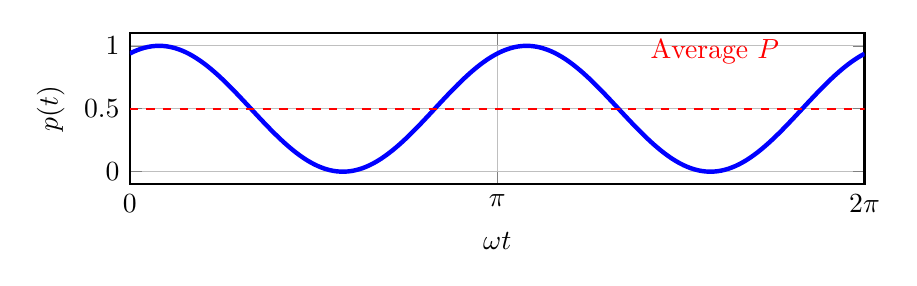
\begin{tikzpicture}
            \begin{axis}[
                width=0.9\textwidth,
                height=3.5cm,
                xlabel={$\omega t$},
                ylabel={$p(t)$},
                xmin=0, xmax=6.28,
                grid=major,
                thick,
                xtick={0, 3.14, 6.28},
                xticklabels={0, $\pi$, $2\pi$}
            ]
            \addplot[blue, ultra thick, domain=0:6.28, samples=200] 
                {0.5 + 0.5*cos(deg(2*x - 0.5))};
            \addplot[red, dashed, domain=0:6.28] {0.5};
            \node[red] at (axis cs: 5,0.95) {Average $P$};
            \end{axis}
        \end{tikzpicture}
        \end{figure}
        
    \end{columns}
    
\end{frame}

\begin{frame}{Reactive and Apparent Power}
    
    \begin{columns}[t]
    \column{0.48\textwidth}
        \textbf{Power Components}:
        
        \textbf{1. Real (Average) Power}:
        \[
        P = V_{rms} I_{rms} \cos\theta \quad \text{(W)}
        \]

        \vspace{-0.1cm}

        \begin{itemize}
            \item Power dissipated (resistors)
        \end{itemize}
        
        \textbf{2. Reactive Power}: 
        \[
        Q = V_{rms} I_{rms} \sin\theta \quad \text{(VAR)}
        \]

        \vspace{-0.1cm}

        \begin{itemize}
            \item Power stored/returned (L/C)
        \end{itemize}
        
        \textbf{3. Apparent Power}: 
        \[
        S = V_{rms} I_{rms} \quad \text{(VA)}
        \]
        
    \column{0.48\textwidth}
        \textbf{Power Triangle}:
        
        \begin{figure}[htb]
        \centering
        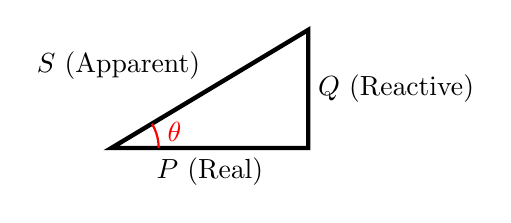
\begin{tikzpicture}[scale=1.0]
            % Triangle
            \draw[ultra thick] (0,0) -- (2.5,0) -- (2.5,1.5) -- cycle;
            
            % Labels
            \node[below] at (1.25,0) {$P$ (Real)};
            \node[right] at (2.5,0.75) {$Q$ (Reactive)};
            \node[above left] at (1.25,0.75) {$S$ (Apparent)};
            
            % Angle
            \draw[red, thick] (0.6,0) arc (0:31: 0.6);
            \node[red] at (0.8,0.2) {$\theta$};
        \end{tikzpicture}
        \end{figure}
        
        \vspace{-0.2cm}
        
        \[
        S = \sqrt{P^2 + Q^2}
        \]
        \[
        P = S \cos\theta, \quad Q = S \sin\theta
        \]
        
        \textbf{Power Factor}:
        \[
        \text{pf} = \cos\theta = \frac{P}{S}
        \]
        
    \end{columns}
    
\end{frame}

\begin{frame}{Power Factor and Its Importance}
    
    \begin{columns}[t]
    \column{0.48\textwidth}
        \textbf{Power Factor Definition}:
        \[
        \text{pf} = \cos\theta = \frac{P}{S}
        \]
        
        Range: $0 \leq \text{pf} \leq 1$
        
        \vspace{0.3cm}
        
        \textbf{Special Cases}:
        \begin{itemize}
            \item[\gooditem] \textbf{pf = 1} (unity): purely resistive, $\theta = 0°$
            \item[\baditem] \textbf{pf = 0}:  purely reactive, $\theta = \pm 90°$
        \end{itemize}
        
        \vspace{0.3cm}
        
        \textbf{Leading vs.  Lagging}:
        \begin{itemize}
            \item Lagging pf: inductive load (current lags voltage)
            \item Leading pf: capacitive load (current leads voltage)
        \end{itemize}
        
    \column{0.48\textwidth}
        
        \begin{block}{Low Power Factor Problems}
            \begin{itemize}
                \item[\baditem] Higher current required
                \item[\baditem] Larger conductor sizes needed
                \item[\baditem] More I\textsuperscript{2}R losses in transmission
            \end{itemize}
        \end{block}
        
        \vspace{0.3cm}
        
        \textbf{Power Factor Correction}:
        
        Add capacitors in parallel with inductive loads to:
        \begin{itemize}
            \item[\gooditem] Increase power factor
            \item[\gooditem] Reduce reactive power
            \item[\gooditem] Lower current draw
        \end{itemize}
        
    \end{columns}
    
\end{frame}

\begin{frame}{Power in Circuit Elements}
    
    \begin{table}
    \centering
    \renewcommand{\arraystretch}{2.2}
    \begin{tabular}{|c|c|c|c|c|}
    \hline
    \textbf{Element} & \textbf{Phase} & \textbf{Real Power $P$} & \textbf{Reactive Power $Q$} & \textbf{pf} \\
    \hline
    \hline
    Resistor & $\theta = 0°$ & $I^2 R$ & 0 & 1 \\
    \hline
    Inductor & $\theta = 90°$ & 0 & $I^2 X_L$ (positive) & 0 \\
    \hline
    Capacitor & $\theta = -90°$ & 0 & $-I^2 X_C$ (negative) & 0 \\
    \hline
    \end{tabular}
    \end{table}
    
    \begin{block}{Key Observations}
        \begin{itemize}
            \item Only \textbf{resistors} dissipate real power (convert to heat $\cdot$ or light if you mess up)
            \item \textbf{Inductors} and \textbf{capacitors} store and return energy (reactive power)
            \item Reactive power from L and C have opposite signs (can cancel to form resonant networks)
        \end{itemize}
    \end{block}
    
    \vspace{0.3cm}
    
    \begin{alertblock}{Complex Power}
        Complex power combines real and reactive:  $\mathbf{S} = P + jQ = \mathbf{V}_{rms}\mathbf{I}^*_{rms}$
    \end{alertblock}
    
\end{frame}

\section{Summary}

\begin{frame}{Summary:  Frequency Domain Analysis}
    
    \begin{columns}[t]
    \column{0.48\textwidth}
        \textbf{Phasor Analysis}:
        \begin{itemize}
            \item Transform:  $V_m\cos(\omega t + \phi) \leftrightarrow V_m\angle\phi$
            \item[\gooditem] Differential equations $\rightarrow$ algebra
            \item $d/dt \rightarrow j\omega$, $\int dt \rightarrow 1/(j\omega)$
        \end{itemize}
        
        \textbf{Impedance}:
        \begin{itemize}
            \item $\mathbf{Z} = R + jX$
            \item Resistor: $\mathbf{Z}_R = R$
            \item Inductor: $\mathbf{Z}_L = j\omega L$
            \item Capacitor: $\mathbf{Z}_C = 1/(j\omega C)$
        \end{itemize}
        
        \textbf{Circuit Analysis}:
        \begin{itemize}
            \item[\gooditem] All DC techniques apply
            \item KVL, KCL, voltage/current dividers
            \item Series/parallel combinations
        \end{itemize}
        
    \column{0.48\textwidth}
        \textbf{AC Power}:
        \begin{itemize}
            \item Real power: $P = V_{rms}I_{rms}\cos\theta$ 
            \item Reactive power: $Q = V_{rms}I_{rms}\sin\theta$ 
            \item Apparent power: $S = V_{rms}I_{rms}$ 
        \end{itemize}
        
        \textbf{Power Factor}:
        \begin{itemize}
            \item $\text{pf} = \cos\theta = P/S$
            \item Lagging pf: inductive
            \item Leading pf: capacitive
            \item[\baditem] Low pf $\rightarrow$ higher losses
        \end{itemize}
        
        \textbf{Resonance}:
        \begin{itemize}
            \item Occurs when $X_L = X_C$
            \item $\omega_0 = 1/\sqrt{LC}$
            \item[\gooditem] Minimum Z, maximum I
        \end{itemize}
        
    \end{columns}
    
\end{frame}

\begin{frame}{Comparison:  Time vs. Frequency Domain}
    
    \begin{table}
    \centering
    \renewcommand{\arraystretch}{1.8}
    \small
    \begin{tabular}{|p{0.25\textwidth}|p{0.32\textwidth}|p{0.32\textwidth}|}
    \hline
    \textbf{Aspect} & \textbf{Time Domain} & \textbf{Frequency Domain} \\
    \hline
    \hline
    Signals & $v(t)$, $i(t)$ (real functions) & $\mathbf{V}$, $\mathbf{I}$ (complex phasors) \\
    \hline
    Math & Differential equations & Algebraic equations \\
    \hline
    Circuit elements & R, L, C (time relations) & $\mathbf{Z}_R$, $\mathbf{Z}_L$, $\mathbf{Z}_C$ (impedances) \\
    \hline
    Analysis & Initial conditions, transients & Steady-state, magnitude/phase \\
    \hline
    Advantages & Shows time evolution & Simplifies sinusoidal analysis \\
    \hline
    Limitations & Complex for AC steady-state & Only sinusoidal steady-state \\
    \hline
    \end{tabular}
    \end{table}
    
    \vspace{-0.2cm}
    
    \begin{block}{When to Use Each}
        \textbf{Time Domain}:  Transients, switching, initial conditions, non-sinusoidal signals\\
        \textbf{Frequency Domain}: AC steady-state, sinusoidal sources, impedance analysis
    \end{block}
    
\end{frame}


% \section{Phasor Basics Problems}

% \begin{frame}{Example 1: Phasor Conversions}
    
%     \textbf{Problem}:  Convert the following time-domain signals to phasors, then perform the operations.
    
%     \vspace{0.3cm}
    
%     \begin{columns}[t]
%     \column{0.48\textwidth}
%         \textbf{Given}:
%         \begin{align*}
%         v_1(t) &= 10\cos(1000t + 30°)\text{ V}\\
%         v_2(t) &= 5\cos(1000t - 45°)\text{ V}\\
%         i(t) &= 2\cos(1000t + 60°)\text{ A}
%         \end{align*}
        
%         \textbf{Find}:
%         \begin{enumerate}
%             \item Phasor forms of $v_1$, $v_2$, and $i$
%             \item $\mathbf{V}_1 + \mathbf{V}_2$
%             \item $\mathbf{V}_1 - \mathbf{V}_2$
%             \item $\mathbf{V}_1 / \mathbf{I}$
%         \end{enumerate}
        
%     \column{0.48\textwidth}
        
        

%         \ifthenelse{\boolean{showresults}}{

%             \vspace{-1cm}    
%             \textbf{Solution}:
            
%             \textbf{Part 1}:  Phasor forms
%             \begin{align*}
%             \mathbf{V}_1 &= 10\angle 30°\text{ V}\\
%             \mathbf{V}_2 &= 5\angle -45°\text{ V}\\
%             \mathbf{I} &= 2\angle 60°\text{ A}
%             \end{align*}
            
%             \pause

%             \vspace{-0.2cm}

%             \textbf{Part 2}: $\mathbf{V}_1 + \mathbf{V}_2$
            
%             Convert to rectangular: 
%             \begin{align*}
%             \mathbf{V}_1 &= 10\cos(30°) + j10\sin(30°)\\
%             &= 8.66 + j5.00\text{ V}\\
%             \mathbf{V}_2 &= 5\cos(-45°) + j5\sin(-45°)\\
%             &= 3.54 - j3.54\text{ V}
%             \end{align*}
%         }{}
        
%     \end{columns}
    
% \end{frame}

% \ifthenelse{\boolean{showresults}}{
% \begin{frame}{Example 1: Solution (continued)}
    
%     \begin{columns}[t]
%     \column{0.48\textwidth}
%         \textbf{Part 2 (continued)}:
%         \begin{align*}
%         \mathbf{V}_1 + \mathbf{V}_2 &= (8.66 + j5.00) + (3.54 - j3.54)\\
%         &= 12.20 + j1.46\text{ V}
%         \end{align*}
        
%         Convert to polar:
%         \begin{align*}
%         |\mathbf{V}| &= \sqrt{12.20^2 + 1.46^2} = 12.29\text{ V}\\
%         \angle\mathbf{V} &= \tan^{-1}\left(\frac{1.46}{12.20}\right) = 6.83°
%         \end{align*}
        
%         \[
%         \boxed{\mathbf{V}_1 + \mathbf{V}_2 = 12.29\angle 6.83°\text{ V}}
%         \]
        
%     \column{0.48\textwidth}
%         \textbf{Part 3}: $\mathbf{V}_1 - \mathbf{V}_2$
%         \begin{align*}
%         \mathbf{V}_1 - \mathbf{V}_2 &= (8.66 + j5.00) - (3.54 - j3.54)\\
%         &= 5.12 + j8.54\text{ V}\\
%         &= 9.96\angle 59.05°\text{ V}
%         \end{align*}
        
%         \[
%         \boxed{\mathbf{V}_1 - \mathbf{V}_2 = 9.96\angle 59.05°\text{ V}}
%         \]
        
%         \textbf{Part 4}: $\mathbf{V}_1 / \mathbf{I}$ (This is impedance!)
%         \begin{align*}
%         \frac{\mathbf{V}_1}{\mathbf{I}} &= \frac{10\angle 30°}{2\angle 60°} = \frac{10}{2}\angle(30° - 60°)\\
%         &= 5\angle -30°\,\Omega
%         \end{align*}

%         \vspace{-0.6cm}
        
%         \[
%         \boxed{\mathbf{Z} = 5\angle -30°\,\Omega = 4.33 - j2.50\,\Omega}
%         \]
        
%     \end{columns}
    
% \end{frame}
% }{}

% \section{Impedance Calculation Problems}

% \begin{frame}{Example 2: Impedance at Different Frequencies}
    
%     \textbf{Problem}:  A series circuit contains $R = 50\,\Omega$, $L = 20$ mH, and $C = 10\,\mu$F. Find the total impedance at the following frequencies.  
    
%     \vspace{0.5cm}
    
%     \begin{columns}[t]
%     \column{0.48\textwidth}
%         \textbf{Circuit}:
        
%         \begin{figure}[htb]
%         \centering
%         \begin{circuitikz}[scale=0.8]
%             \draw (0,0) to[short, o-] (0.5,0);
%             \draw (0.5,0) to[R, l=$50\,\Omega$] (2,0);
%             \draw (2,0) to[L, l=$20$ mH] (3. 5,0);
%             \draw (3.5,0) to[C, l=$10\,\mu$F] (5,0);
%             \draw (5,0) to[short, -o] (5.5,0);
%         \end{circuitikz}
%         \end{figure}
        
%         \textbf{Given}:
%         \begin{itemize}
%             \item $R = 50\,\Omega$
%             \item $L = 20$ mH
%             \item $C = 10\,\mu$F
%         \end{itemize}
        
%     \column{0.48\textwidth}
%         \textbf{Find the total impedance at}:
%         \begin{itemize}
%             \item (a) $f = 100$ Hz
%             \item (b) $f = 500$ Hz
%             \item (c) $f = 1000$ Hz
%         \end{itemize}
        
%         \vspace{1cm}
        
%         \textbf{For each frequency, determine}:
%         \begin{enumerate}
%             \item Magnitude $|\mathbf{Z}|$
%             \item Phase angle $\theta$
%             \item Whether the circuit is inductive or capacitive
%         \end{enumerate}
        
%     \end{columns}
    
% \end{frame}

% \ifthenelse{\boolean{showresults}}{
% \begin{frame}{Example 2: Solution - Setup and Part (a)}
    
%     \textbf{General Formula for Series RLC}:
%     \[
%     \mathbf{Z} = R + j\omega L + \frac{1}{j\omega C} = R + j\left(\omega L - \frac{1}{\omega C}\right)
%     \]
    
%     where $X_L = \omega L$ (inductive reactance) and $X_C = \dfrac{1}{\omega C}$ (capacitive reactance)

%     \textbf{Part (a): $f = 100$ Hz}
    
%     \begin{columns}[t]
%     \column{0.48\textwidth}
%         % Calculate $\omega$:
%         \[
%         \omega = 2\pi f = 2\pi(100) = 628.3\text{ rad/s}
%         \]
        
%         % Calculate reactances:
%         \begin{align*}
%         X_L &= \omega L = 628.3 \times 0.02 = 12.57\,\Omega
%         \end{align*}
%         \begin{align*}
%         X_C &= \frac{1}{\omega C} = \frac{1}{628.3 \times 10^{-5}} = 159.2\,\Omega
%         \end{align*}
        
%     \column{0.48\textwidth}
%         % Net reactance:
%         \begin{align*}
%         X &= X_L - X_C = -146.6\,\Omega
%         \end{align*}

%         \vspace{-0.5cm}

%         \[
%         \mathbf{Z} = 50 - j146.6\,\Omega
%         \]

%         \vspace{-0.5cm}
        
%         \[
%         \boxed{\mathbf{Z} = 154.9\angle -71.2°\,\Omega}
%         \]
        
%         \textit{Capacitive behavior (negative reactance, current leads)}
        
%     \end{columns}
    
% \end{frame}
% }{}

% \ifthenelse{\boolean{showresults}}{
% \begin{frame}{Example 2: Solution - Parts (b) and (c)}
    
%     \begin{columns}[t]
%     \column{0.48\textwidth}
%         \textbf{Part (b): $f = 500$ Hz}
        
%         $\omega = 2\pi(500) = 3141.6$ rad/s
        
%         \begin{align*}
%         X_L &= 3141.6 \times 0.02 = 62.83\,\Omega\\
%         X_C &= \frac{1}{3141.6 \times 10^{-5}} = 31.83\,\Omega\\
%         X &= 62.83 - 31.83 = 31.0\,\Omega
%         \end{align*}
        
%         \[
%         \mathbf{Z} = 50 + j31.0\,\Omega
%         \]
        
%         \[
%         \boxed{\mathbf{Z} = 59.0\angle 31.8°\,\Omega}
%         \]
        
%         \textit{Inductive behavior (positive reactance, current lags)}
        
%     \column{0.48\textwidth}
%         \textbf{Part (c): $f = 1000$ Hz}
        
%         $\omega = 2\pi(1000) = 6283.2$ rad/s
        
%         \begin{align*}
%         X_L &= 6283.2 \times 0.02 = 125.7\,\Omega\\
%         X_C &= \frac{1}{6283.2 \times 10^{-5}} = 15.92\,\Omega\\
%         X &= 125.7 - 15.92 = 109.8\,\Omega
%         \end{align*}
        
%         \[
%         \mathbf{Z} = 50 + j109.8\,\Omega
%         \]
        
%         \[
%         \boxed{\mathbf{Z} = 120.7\angle 65.5°\,\Omega}
%         \]
        
%         \textit{Inductive behavior (positive reactance, current lags)}
        
%     \end{columns}
    
%     \vspace{0.5cm}
    
%     \begin{block}{Key Observation}
%         As frequency increases:  $X_L \uparrow$ and $X_C \downarrow$. The circuit transitions from \textbf{capacitive} (100 Hz) to \textbf{inductive} (500 Hz, 1000 Hz). There's a resonant frequency in between where $X_L = X_C$! 
%     \end{block}
    
% \end{frame}
% }{}

% \section{Circuit Analysis }

% \begin{frame}{Example 3: Series RL Circuit}
    
%     \textbf{Problem}:  For the circuit shown, find the current, voltage across each element, and draw the phasor diagram. 
    
%     \vspace{0.5cm}
    
%     \begin{columns}[t]
%     \column{0.48\textwidth}
%         \textbf{Circuit}:
        
%         \begin{figure}[htb]
%         \centering
%         \begin{circuitikz}[scale=0.9]
%             \draw (0,0) to[sinusoidal voltage source, l=$v_s(t)$] (0,3);
%             \draw (0,3) to[R, l=$30\,\Omega$, v_=$v_R$] (2.5,3);
%             \draw (2.5,3) to[L, l=$50$ mH, v_=$v_L$, i^=$i(t)$] (5,3);
%             \draw (5,3) to[short] (5,0);
%             \draw (5,0) to[short] (0,0);
%         \end{circuitikz}
%         \end{figure}
       
%     \column{0.48\textwidth}

%     \vspace{-1cm}

%         \textbf{Given}:
%         \begin{itemize}
%             \item $v_s(t) = 100\cos(2000t)$ V
%             \item $R = 30\,\Omega$
%             \item $L = 50$ mH $= 0.05$ H
%             \item $\omega = 2000$ rad/s
%         \end{itemize}


%         \textbf{Find}:
%         \begin{enumerate}
%             \item Total impedance $\mathbf{Z}_{tot}$
%             \item Current $i(t)$ (phasor and time domain)
%             \item Voltage across resistor $v_R(t)$
%             \item Voltage across inductor $v_L(t)$
%             \item Draw the phasor diagram
%             \item Verify KVL
%         \end{enumerate}
        
%     \end{columns}
    
% \end{frame}

% \ifthenelse{\boolean{showresults}}{
% \begin{frame}{Example 3: Solution - Impedance and Current}
    
%     \begin{columns}[t]
%     \column{0.48\textwidth}
%         \textbf{Step 1: Convert to phasor domain}
        
%         Source phasor: 
%         \[
%         \mathbf{V}_s = 100\angle 0°\text{ V}
%         \]
        
%         \vspace{0.3cm}
        
%         \textbf{Step 2: Calculate impedances}
        
%         Resistor impedance:
%         \[
%         \mathbf{Z}_R = R = 30\,\Omega
%         \]
        
%         Inductor impedance:
%         \begin{align*}
%         \mathbf{Z}_L &= j\omega L\\
%         &= j(2000)(0.05)\\
%         &= j100\,\Omega
%         \end{align*}
        
%     \column{0.48\textwidth}
%         \textbf{Step 3: Total impedance}
        
%         Rectangular form:
%         \[
%         \mathbf{Z}_{tot} = \mathbf{Z}_R + \mathbf{Z}_L = 30 + j100\,\Omega
%         \]
        
%         Polar form: 
%         \begin{align*}
%         |\mathbf{Z}_{tot}| &= \sqrt{30^2 + 100^2} = 104.4\,\Omega
%         \end{align*}
%         \begin{align*}
%         \theta_Z &= \tan^{-1}\left(\frac{100}{30}\right) = 73.3°
%         \end{align*}
        
%         \[
%         \boxed{\mathbf{Z}_{tot} = 104.4\angle 73.3°\,\Omega}
%         \]
        
%     \end{columns}
    
% \end{frame}
% }{}

% \ifthenelse{\boolean{showresults}}{
% \begin{frame}{Example 3: Solution - Current (continued)}
    
%     \begin{columns}[t]
%     \column{0.48\textwidth}
%         \textbf{Step 4: Calculate current}
        
%         Using Ohm's law:
%         \begin{align*}
%         \mathbf{I} &= \frac{\mathbf{V}_s}{\mathbf{Z}_{tot}}\\
%         &= \frac{100\angle 0°}{104.4\angle 73.3°}\\
%         &= \frac{100}{104.4}\angle(0° - 73.3°)\\
%         &= 0.958\angle -73.3°\text{ A}
%         \end{align*}
        
%         \[
%         \boxed{\mathbf{I} = 0.958\angle -73.3°\text{ A}}
%         \]
        
%     \column{0.48\textwidth}
%         \textbf{Step 5: Convert to time domain}
        
%         \[
%         \boxed{i(t) = 0.958\cos(2000t - 73.3°)\text{ A}}
%         \]
        
%         \vspace{0.5cm}
        
%         \begin{block}{Interpretation}
%             Current \textbf{lags} the voltage by $73.3°$, which is expected for an inductive circuit (RL circuit).
%         \end{block}
        
%     \end{columns}
    
% \end{frame}
% }{}

% \ifthenelse{\boolean{showresults}}{
% \begin{frame}{Example 3: Solution - Element Voltages}
    
%     \begin{columns}[t]
%     \column{0.48\textwidth}
%         \textbf{Step 6: Voltage across resistor}
        
%         Using Ohm's law:
%         \begin{align*}
%         \mathbf{V}_R &= \mathbf{I} \cdot \mathbf{Z}_R\\
%         &= (0.958\angle -73.3°)(30\angle 0°)\\
%         &= 0.958 \times 30 \angle(-73.3° + 0°)\\
%         &= 28.7\angle -73.3°\text{ V}
%         \end{align*}
        
%         \[
%         \boxed{\mathbf{V}_R = 28.7\angle -73.3°\text{ V}}
%         \]
        
%         Time domain:
%         \[
%         v_R(t) = 28.7\cos(2000t - 73.3°)\text{ V}
%         \]
        
%         \textit{Note: $\mathbf{V}_R$ is in phase with $\mathbf{I}$ (both at $-73.3°$)}
        
%     \column{0.48\textwidth}
%         \textbf{Step 7: Voltage across inductor}
        
%         Using Ohm's law:
%         \begin{align*}
%         \mathbf{V}_L &= \mathbf{I} \cdot \mathbf{Z}_L\\
%         &= (0.958\angle -73.3°)(100\angle 90°)\\
%         &= 0.958 \times 100 \angle(-73.3° + 90°)\\
%         &= 95.8\angle 16.7°\text{ V}
%         \end{align*}
        
%         \[
%         \boxed{\mathbf{V}_L = 95.8\angle 16.7°\text{ V}}
%         \]
        
%         Time domain:
%         \[
%         v_L(t) = 95.8\cos(2000t + 16.7°)\text{ V}
%         \]
        
%         \textit{Note:  $\mathbf{V}_L$ leads $\mathbf{I}$ by $90°$ (as expected for an inductor)}
        
%     \end{columns}
    
% \end{frame}
% }{}

% \ifthenelse{\boolean{showresults}}{
% \begin{frame}{Example 3: Solution - Phasor Diagram and Verification}
    
%     \begin{columns}[t]
%     \column{0.48\textwidth}
%         \textbf{Step 8: Verify KVL}
        
%         Check:  $\mathbf{V}_R + \mathbf{V}_L = \mathbf{V}_s$
        
%         Convert to rectangular: 
%         \begin{align*}
%         \mathbf{V}_R &= 28.7\angle -73.3°\\
%         &= 28.7\cos(-73.3°) + j28.7\sin(-73.3°)\\
%         &= 8.26 - j27.49\text{ V}
%         \end{align*}

%         \vspace{-0.8cm}
        
%         \begin{align*}
%         \mathbf{V}_L &= 95.8\angle 16.7°\\
%         &= 95.8\cos(16.7°) + j95.8\sin(16.7°)\\
%         &= 91.74 + j27.49\text{ V}
%         \end{align*}

%         \vspace{-0.8cm}
        
%         \begin{align*}
%         \mathbf{V}_R + \mathbf{V}_L &= (8.26 - j27.49) + (91.74 + j27.49)\\
%         &= 100 + j0 = 100\angle 0°\text{ V} \;
%         \end{align*}
        
%     \column{0.48\textwidth}
        
%         \vspace{-0.75cm}
        
%         \begin{figure}[htb]
%         \centering
%         \begin{tikzpicture}[scale=0.7]
%             % Axes
%             \draw[->] (-1,0) -- (4,0) node[right] {Re};
%             \draw[->] (0,-2.5) -- (0,2.5) node[above] {Im};
            
%             % Vs (reference)
%             \draw[->, ultra thick, black] (0,0) -- (3,0) node[midway, below] {$\mathbf{V}_s$};
            
%             % I (lags by 73.3°)
%             \draw[->, ultra thick, green! 60!black] (0,0) -- (0.3,-0.95) node[right] {$\mathbf{I}$};
            
%             % VR (parallel to I)
%             \draw[->, ultra thick, blue] (0,0) -- (0.86,-2.74) node[below right] {$\mathbf{V}_R$};
            
%             % VL (leads I by 90°, so 16.7° total)
%             \draw[->, ultra thick, red] (0,0) -- (2.88,0.82) node[above right] {$\mathbf{V}_L$};
            
%             % Vector addition:  VR + VL = Vs
%             \draw[dashed, purple] (0.86,-2.74) -- (3,0);
%             \draw[dashed, purple] (2.88,0.82) -- (3,0);
            
%             % Angle markers
%             \draw[green!60!black, thick] (0.5,0) arc (0:-73.3:0.5);
%             \node[green!60!black] at (0.6,-0.4) {\small $-73.3°$};
%         \end{tikzpicture}
%         \end{figure}
        
%         \vspace{-0.6cm}
        
%         \begin{block}{Key Observations}
%             \begin{itemize}
%                 \item $\mathbf{V}_R \parallel \mathbf{I}$ (resistor)
%                 \item $\mathbf{V}_L \perp \mathbf{I}$, leads by $90°$ (inductor)
%                 \item $\mathbf{V}_R + \mathbf{V}_L = \mathbf{V}_s$ (KVL)
%             \end{itemize}
%         \end{block}
        
%     \end{columns}
    
% \end{frame}
% }{}


% \begin{frame}{Example 4: RC Voltage Divider}
    
%     \textbf{Problem}:  Analyze the following RC voltage divider circuit. 
    
%     \vspace{0.3cm}
    
%     \begin{columns}[t]
%     \column{0.48\textwidth}
%         \textbf{Circuit}: 
        
%         \begin{figure}[htb]
%         \centering
%         \begin{circuitikz}[scale=0.9]
%             \draw (0,0) to[sinusoidal voltage source, l=$v_s(t)$] (0,3.5);
%             \draw (0,3.5) to[R, l=$1$ k$\Omega$, i^=$i(t)$] (0,5.5);
%             \draw (0,5.5) to[short] (3,5.5);
%             \draw (3,5.5) to[C, l_=$100$ nF, v^=$v_o(t)$] (3,3.5);
%             \draw (3,3.5) to[short] (3,0);
%             \draw (3,0) to[short] (0,0);
%             \draw (3,3.5) to[short, -o] (4,3.5);
%             \draw (3,5.5) to[short, -o] (4,5.5);
%         \end{circuitikz}
%         \end{figure}
        

%     \column{0.48\textwidth}

%     \vspace{-0.7cm}

%         \textbf{Given}:
%         \begin{itemize}
%             \item $v_s(t) = 10\cos(10000t)$ V
%             \item $R = 1$ k$\Omega$
%             \item $C = 100$ nF
%         \end{itemize}
        
%         \textbf{Find}:
%         \begin{enumerate}
%             \item The impedance of each element
%             \item The output voltage $\mathbf{V}_o$ 
%             \item The output voltage $v_o(t)$ 
%             \item The magnitude ratio $|\mathbf{V}_o|/|\mathbf{V}_s|$
%             \item The phase shift between input and output
%             \item The current $i(t)$
%         \end{enumerate}
        
      
        
%     \end{columns}
    
% \end{frame}

% \ifthenelse{\boolean{showresults}}{
% \begin{frame}{Example 4: Solution}
    
%     \begin{columns}[t]
%     \column{0.48\textwidth}
%         \textbf{Solution}:
        
%         Source phasor: $\mathbf{V}_s = 10\angle 0°$ V
        
%         $\omega = 10000$ rad/s

%         \vspace{1cm}
        
%         \textbf{1. Impedances}:
%         \begin{align*}
%         \mathbf{Z}_R &= 1000\,\Omega\\
%         \mathbf{Z}_C &= \frac{1}{j\omega C} = \frac{1}{j(10^4)(10^{-7})} = -j1000\,\Omega
%         \end{align*}
        
%         \vspace{1cm}
        
%     \column{0.48\textwidth}

%         \textbf{2. Output Voltage (voltage divider)}

    
%         \begin{align*}
%         \mathbf{V}_o &= \mathbf{V}_s \frac{\mathbf{Z}_C}{\mathbf{Z}_R + \mathbf{Z}_C}\\
%         &= 10\angle 0° \cdot \frac{-j1000}{1000 - j1000}
%         \end{align*}


%         \begin{align*}
%         &= 10 \cdot \frac{1000\angle -90°}{1414.2\angle -45°}\\
%         &= 10 \cdot 0.707\angle -45°\\
%         &= \boxed{7.07\angle -45°\text{ V}}
%         \end{align*}
        
        
%     \end{columns}
    
% \end{frame}
% }{}

% \ifthenelse{\boolean{showresults}}{
% \begin{frame}{Example 4: Solution (continued)}
    
%     \begin{columns}[t]
%     \column{0.48\textwidth}

%         \textbf{3. Time domain}:
%         \[
%         \boxed{v_o(t) = 7.07\cos(10000t - 45°)\text{ V}}
%         \]
        
%         \textbf{4. Magnitude ratio}:
%         \[
%         \boxed{\frac{|\mathbf{V}_o|}{|\mathbf{V}_s|} = \frac{7.07}{10} = 0.707}
%         \]

%         \textbf{5. Phase shift}:  $\boxed{-45°}$ (output lags input)

%     \column{0.48\textwidth}
        
%         \textbf{6. Current}:
%         \begin{align*}
%         \mathbf{I} &= \frac{\mathbf{V}_s}{\mathbf{Z}_R + \mathbf{Z}_C} = \frac{10\angle 0°}{1414.2\angle -45°}\\
%         &= 7.07\angle 45°\text{ mA}
%         \end{align*}
%         \[
%         \boxed{i(t) = 7.07\cos(10000t + 45°)\text{ mA}}
%         \]
        
%     \end{columns}
    
% \end{frame}
% }{}

% \section{AC Power Problems}

% \begin{frame}{Example 5: AC Power Calculation}
    
%     \textbf{Problem}:  Calculate the real, reactive, and apparent power for a load with the following voltage and current.   
    
%     \vspace{0.5cm}
    
%     \begin{columns}[t]
%     \column{0.48\textwidth}
%         \textbf{Given}:
%         \begin{align*}
%         v(t) &= 120\sqrt{2}\cos(377t)\text{ V}\\
%         i(t) &= 10\sqrt{2}\cos(377t - 36.87°)\text{ A}
%         \end{align*}
        
%         \vspace{0.5cm}
        
%         \textit{Note:   The coefficients include $\sqrt{2}$ to indicate peak values}
        
%     \column{0.48\textwidth}
%         \textbf{Find}:
%         \begin{enumerate}
%             \item RMS voltage and current
%             \item Real power $P$
%             \item Reactive power $Q$
%             \item Apparent power $S$
%             \item Power factor (and type)
%             \item Load impedance $\mathbf{Z}$
%         \end{enumerate}
        
%     \end{columns}
    
% \end{frame}

% \ifthenelse{\boolean{showresults}}{
% \begin{frame}{Example 5: Solution - RMS Values and Powers}
    
%     \begin{columns}[t]
%     \column{0.48\textwidth}
%         \textbf{Step 1: RMS values}
        
%         Convert from peak to RMS:
%         \begin{align*}
%         V_{rms} &= \frac{V_m}{\sqrt{2}} = \frac{120\sqrt{2}}{\sqrt{2}} = \boxed{120\text{ V}}
%         \end{align*}

%         \vspace{-0.6cm}
        
%         \begin{align*}
%         I_{rms} &= \frac{I_m}{\sqrt{2}} = \frac{10\sqrt{2}}{\sqrt{2}} = \boxed{10\text{ A}}
%         \end{align*}
        
%         \vspace{-0.3cm}
        
%         \textbf{Step 2: Determine phase angle}
        
%         From the time-domain expressions:
%         \begin{itemize}
%             \item Voltage phase: $\phi_v = 0°$
%             \item Current phase: $\phi_i = -36.87°$
%         \end{itemize}
        
%         Phase difference: 
%         \[
%         \theta = \phi_v - \phi_i = 0° - (-36.87°) = 36.87°
%         \]

%         \vspace{-0.3cm}
        
%         \textit{Current lags voltage $\Rightarrow$ inductive load}
        
%     \column{0.48\textwidth}
%         \textbf{Step 3: Real power}
%         \begin{align*}
%         P &= V_{rms} I_{rms} \cos\theta\\
%         &= (120)(10)\cos(36.87°) = \boxed{960\text{ W}}
%         \end{align*}
        
%         \textbf{Step 4: Reactive power}
%         \begin{align*}
%         Q &= V_{rms} I_{rms} \sin\theta\\
%         &= (120)(10)\sin(36.87°) = \boxed{720\text{ VAR}}
%         \end{align*}
        
%         % \textit{Positive $Q$ confirms inductive load}
        
%         \textbf{Step 5: Apparent power}
%         \begin{align*}
%         S &= V_{rms} I_{rms}  = \boxed{1200\text{ VA}}
%         \end{align*}
        
%         \textbf{Verify}:  $S = \sqrt{P^2 + Q^2} = \sqrt{960^2 + 720^2} = 1200$ 
        
%     \end{columns}
    
% \end{frame}
% }{}

% \ifthenelse{\boolean{showresults}}{
% \begin{frame}{Example 5: Solution - Power Factor and Impedance}
    
%     \begin{columns}[t]
%     \column{0.48\textwidth}
%         \textbf{Step 6: Power factor}
        
%         Method 1 - From angle:
%         \begin{align*}
%         \text{pf} &= \cos\theta = \cos(36.87°)\\
%         &= \boxed{0.8\text{ lagging}}
%         \end{align*}
        
%         Method 2 - From powers:
%         \begin{align*}
%         \text{pf} &= \frac{P}{S} = \frac{960}{1200}\\
%         &= 0.8\text{ lagging}
%         \end{align*}
        
%         \textit{``Lagging'' because current lags voltage (inductive)}
        
%     \column{0.48\textwidth}
%         \textbf{Step 7: Load impedance}
        
%         Convert to phasor form:

%         \vspace{-0.6cm}
        
%         \begin{align*}
%         \mathbf{V} &= 120\angle 0°\text{ V}\\
%         \mathbf{I} &= 10\angle -36.87°\text{ A}
%         \end{align*}
        
%         Calculate impedance:
%         \begin{align*}
%         \mathbf{Z} &= \frac{\mathbf{V}}{\mathbf{I}} = \frac{120\angle 0°}{10\angle -36.87°}\\
%         &= 12\angle 36.87°\,\Omega
%         \end{align*}
        
%         \vspace{-1cm}

%         \begin{align*}
%         \mathbf{Z} &= 12(\cos 36.87° + j\sin 36.87°)\\
%         &= \boxed{9.6 + j7.2\,\Omega}
%         \end{align*}
        
%         \textit{This represents $R = 9.6\,\Omega$ in series with $X_L = 7.2\,\Omega$}
        
%     \end{columns}
    
% \end{frame}
% }{}

% \begin{frame}{Example 6: Parallel RLC Circuit}
    
%     \textbf{Problem}: Analyze the parallel RLC circuit shown below.
    
%     \vspace{0.3cm}
    
%     \begin{columns}[t]
%     \column{0.48\textwidth}
%         \textbf{Circuit}:
        
%         \begin{figure}[htb]
%         \centering
%         \begin{circuitikz}[scale=0.85]
%             \draw (0,0) to[sinusoidal voltage source, l=$v_s(t)$, i=$i_s$] (0,4);
%             \draw (0,4) to[short] (1,4);
%             \draw (1,4) to[R, l=$200\,\Omega$, i^=$i_R$, *-*] (1,0);
%             \draw (2.5,4) to[L, l=$0.5$ H, i^=$i_L$, *-*] (2.5,0);
%             \draw (4,4) to[C, l=$5\,\mu$F, i^=$i_C$, *-*] (4,0);
%             \draw (1,4) to[short] (2.5,4);
%             \draw (2.5,4) to[short] (4,4);
%             \draw (1,0) to[short] (2.5,0);
%             \draw (2.5,0) to[short] (4,0);
%             \draw (4,0) to[short] (5,0);
%             \draw (0,0) to[short] (1,0);
%         \end{circuitikz}
%         \end{figure}
        

        
%     \column{0.48\textwidth}

%         \textbf{Given}:
%         \begin{itemize}
%             \item $v_s(t) = 50\cos(1000t)$ V
%         \end{itemize}


%         \textbf{Find}:
%         \begin{enumerate}
%             \item Impedance of each branch
%             \item Total impedance
%             \item Source current $i_s(t)$
%             \item Current through each branch
%             \item Total real power
%             \item Total reactive power
%             \item Is the circuit inductive or capacitive?
%         \end{enumerate}
        
        
%     \end{columns}
    
% \end{frame}

% \ifthenelse{\boolean{showresults}}{
% \begin{frame}{Example 6: Solution}
    
%     \begin{columns}[t]
%     \column{0.48\textwidth}
%         \textbf{Solution}:
        
%         $\mathbf{V}_s = 50\angle 0°$ V, $\omega = 1000$ rad/s
        
%         \textbf{1. Branch impedances}:
%         \begin{align*}
%         \mathbf{Z}_R &= 200\,\Omega\\
%         \mathbf{Z}_L &= j\omega L = j(1000)(0.5) = j500\,\Omega\\
%         \mathbf{Z}_C &= \frac{1}{j\omega C} = \frac{1}{j(1000)(5 \times 10^{-6})}\\
%         &= -j200\,\Omega
%         \end{align*}
        
%         \textbf{2. Total impedance}:
%         \begin{align*}
%         \frac{1}{\mathbf{Z}_{tot}} &= \frac{1}{200} + \frac{1}{j500} + \frac{1}{-j200}\\
%         &=  0.005 + j0.003
%         \end{align*}
        
%     \column{0.48\textwidth}
%         \begin{align*}
%         \mathbf{Z}_{tot} &= \frac{1}{0.005 + j0.003} = \frac{1}{0.00583\angle 30.96°}\\
%         &= \boxed{171.5\angle -30.96°\,\Omega}\\
%         &= 147.1 - j88.0\,\Omega
%         \end{align*}
        
%         \textbf{3. Source current}:
%         \begin{align*}
%         \mathbf{I}_s &= \frac{\mathbf{V}_s}{\mathbf{Z}_{tot}} = \frac{50\angle 0°}{171.5\angle -30.96°}\\
%         &= 0.292\angle 30.96°\text{ A}
%         \end{align*}
%         \[
%         \boxed{i_s(t) = 0.292\cos(1000t + 30.96°)\text{ A}}
%         \]
        

        
%     \end{columns}
    
% \end{frame}
% }{}

% \ifthenelse{\boolean{showresults}}{
% \begin{frame}{Example 6: Solution (continued)}
    
%     \begin{columns}[t]
%     \column{0.48\textwidth}

%         \textbf{4. Branch currents}:
%         \begin{align*}
%         \mathbf{I}_R &= \frac{\mathbf{V}_s}{\mathbf{Z}_R} = \frac{50}{200} = 0.25\angle 0°\text{ A}\\
%         \mathbf{I}_L &= \frac{50\angle 0°}{500\angle 90°} = 0.1\angle -90°\text{ A}\\
%         \mathbf{I}_C &= \frac{50\angle 0°}{200\angle -90°} = 0.25\angle 90°\text{ A}
%         \end{align*}
        
%         \textbf{5. Total real power}:
        
%         Only resistor dissipates real power:
%         \begin{align*}
%         P &= I_R^2 R = \boxed{12.5\text{ W}}
%         \end{align*}

%         \vspace{-0.2cm}
        
%         or using $P = V_{rms} I_{s,rms} \cos\theta$:
%         \begin{align*}
%         P &= 50 \times 0.292 \times \cos(30.96°)= 12.5\text{ W} \;
%         \end{align*}
        
%     \column{0.48\textwidth}
%         \textbf{6. Total reactive power}: 
%         \begin{align*}
%         Q_L &= I_L^2 X_L = (0.1)^2 \times 500 = 5\text{ VAR}\\
%         Q_C &= -I_C^2 X_C = -(0.25)^2 \times 200 = -12.5\text{ VAR}\\
%         Q_{tot} &= Q_L + Q_C = \boxed{-7.5\text{ VAR}}
%         \end{align*}
        
%         or: 
%         \begin{align*}
%         Q &= V_{rms} I_{s,rms} \sin\theta\\
%         &= 50 \times 0.292 \times \sin(30.96°) = -7.5\text{ VAR} \;
%         \end{align*}
        
%         \textbf{7. Circuit behavior}:
        
%         $Q_{tot} < 0$ and current leads voltage ($\theta > 0$)
        
%         \textit{Capacitor reactive power dominates}
        
%     \end{columns}
    
% \end{frame}
% }{}

\end{document}